\documentclass{article}
\usepackage{graphicx}
\usepackage{amsmath}

\begin{document}

\begin{center}
\Large \textbf{GATE Question}

\vspace{0.5cm}

\normalsize
Name: Harshita N Kumar \\
ID: COMETFWC052

\end{center}

\section*{Question}

The logic gate circuit shown in the figure realizes which of the following functions?

\begin{enumerate}
\item XOR
\item XNOR
\item Half Adder
\item Full Adder
\end{enumerate}

\begin{center}
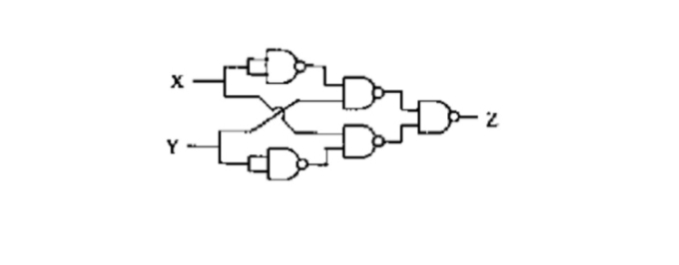
\includegraphics[width=10cm]{question.jpg}
\end{center}

\section*{Solution}

The circuit is composed entirely of NAND gates.

Using NAND implementation:

$$
A = NAND(X,Y)
$$

$$
B = NAND(X,A)
$$

$$
C = NAND(Y,A)
$$

$$
Z = NAND(B,C)
$$

This simplifies to

$$
Z = X \oplus Y
$$

Hence the circuit implements the \textbf{XOR gate}.

\section*{Truth Table}

\begin{center}
\begin{tabular}{|c|c|c|}
\hline
X & Y & Z \\
\hline
0 & 0 & 0 \\
0 & 1 & 1 \\
1 & 0 & 1 \\
1 & 1 & 0 \\
\hline
\end{tabular}
\end{center}

\section*{Graph Output}

\begin{center}

\includegraphics[width=10cm]{graph.jpg}
\end{center}

\end{document}
